\chapter{Grundlagen}
Um die Folgenden Inhalte wie Konzeption und Implementierung aber auch Verwandte Arbeiten nachvollziehen zu können, werden in diesem Kapitel grundlegende Begriffe, Techniken sowie Technologien erläutert.

\section{Definitionen}
    \subsection{Smart Devices} \label{SmartDevices}
        \glqq informationstechnisch aufgerüstete Alltagsgegenstände, die einen Mehrwert durch sensorgestützte Informationsverarbeitung und Kommunikation erhalten.\grqq{} \cite{lackes_siepermann_2018}.
        
        Dieses Zitat von Herr Lakes et al. nennt als Hauptmerkmale eines solchen Geräts, den alltäglichen Einsatz der Gegenstände, welche mithilfe von Sensorik und Kommunikation einen Mehrwert generieren.
        Nimmt man nun ein Gerät, welches als \emph{Smart Device} bezeichnet wird, erkennt man, dass die Aussage zutreffend ist. Als Beispiel wird eine intelligente Steckdose verwendet. Sie ist ein alltäglicher Gegenstand, welcher über Funk angesteuert werden kann. Somit kann ein anderes Gerät, welches sich mit der Steckdose verbinden lässt, den aktuellen Status abfragen oder verändern.
        Hier repräsentiert der Funk den Sensor, welcher in normalen Steckdosen nicht verfügbar ist, und übermittelt den aktuellen Status (Informationen) an ein externes Gerät. Mithilfe dieses Gerätes ist dann eine Steuerung der Steckdose möglich, was einen Mehrwert bietet.
    
    \subsection{Internet der Dinge}
        \glqq bezeichnet die Vernetzung von Gegenständen mit dem Internet, damit diese Gegenstände selbstständig über das Internet kommunizieren und so verschiedene Aufgaben für den Besitzer erledigen können. Der Anwendungsbereich erstreckt sich dabei von einer allg. Informationsversorgung über automatische Bestellungen bis hin zu Warn- und Notfallfunktionen.\grqq{}
        \cite{lackes_siepermann_2018_iot}.
    
        Die Definition des Begriffs \emph{Internet der Dinge} oder \ac{IoT} von Herr Lakes et al. deckt sich in vielen Punkten mit der Definition \ref{SmartDevices}. Hier befinden sich ebenfalls vernetzte Geräte, welche sich untereinander mit Informationen versorgen und somit Aufgaben übernehmen (einen Mehrwert bieten) können. Das Wichtige an diesem Begriff ist der Zusammenschluss solch intelligenter Geräte in größere Netze. Die Geräte müssen dabei nicht gleichartig sein und können unterschiedliche Aufgaben im Alltag übernehmen. Sie können Abhängigkeiten zueinander besitzen und sich gegenseitig Ansprechen oder aktivieren ohne direkte Befehle vom Besitzer, also Nutzer, zu erhalten.
        
        Diese Vorstellung von \ac{IoT} teilt auch Ashton im RFID Journal.
        %http://www.itrco.jp/libraries/RFIDjournal-That%20Internet%20of%20Things%20Thing.pdf
        \grqq If we had computers that knew everything there was to know about things—using data they gathered without any help from us—we would be able to track and count everything, and greatly reduce waste, loss and cost. We would know when things needed replacing, repairing or recalling, and whether they were fresh or past their best.\glqq{} \cite{ashton2009internet}
        Dieses Zitat beschreibt die Motivation, welche hinter dem \emph{Internet der Dinge} steht.
        Im Fokus ist die Automatisierung von Abläufen, ohne Zutun von Menschen. Darüber hinaus bekommen Menschen umfassende Informationen über aktuelle Zustände aller Geräte und können ihre Aktionen besser koordinieren. Dies würde die Abläufe effizienter machen wodurch Geld eingespart und Prozesse optimiert werden können.

\section{MQTT}
    \subsection{Publish/Subscribe}
    Das publish/subscribe Prinzip besteht aus einer Client-Server Architektur, wobei nur der Client aktiv kommuniziert. Er verbindet sich mit dem Server und hält eine Verbindung zu diesem offen, wodurch er die Nachrichten an eine sogenannte Topic, vergleichbar mit einem Postfach im Broker, sendet. Gleichzeitig kann er mehrere angelegte Topics abonnieren (subscriben), was bedeutet, dass er auf diesem Pfad nach neuen Nachrichten lauscht. Sobald sie beim Broker eintrifft, veröffentlicht er diese für die Clients. Anschließend können diese die Informationen der Mitteilungen verarbeiten.

    Dieses Prinzip ermöglicht eine Kommunikation zwischen Geräten, welche keine gute Verbindung besitzen oder eine niedrige Bandbreite einhalten müssen. Im Gegensatz zu dem Request/Response Prinzip, welches unter anderem bei Webseiten verwendet wird, ist es hier nicht nötig sogenannte \glqq Update-Requests\grqq{} zu senden, da die Verbindung offen gehalten wird.
    Diese Eigenschaft eignet sich besonders für \emph{Smart Devices} oder Geräte die nur wenig Informationen bei Bedarf senden müssen oder wenig Rechenkraft besitzen.
    %TODO: \cite{}

    \subsection{Standard}
        \ac{MQTT} oder auch Message Queue Telemetry Transport ist ein Protokoll, welches auf dem zuvor beschriebenen Publish/Subscribe Prinzip basiert. Es wurde ursprünglich zwischen 1998-1999 von IBM und Arcom (heute Eurotech) entwickelt. Die Version 3.1.1 wurde Ende 2014 als OASIS Standard verabschiedet und ist bis heute noch der De-Facto-Standard. Dies ist ebenfalls anhand des ISO/IEC 20922 Standards zu erkennen, wodurch das Protokoll in 2016 aufgenommen wurde. \cite{eclipse_foundation2017} Mitte 2019 wurde die Version 5.0 ebenfalls als OASIS Standard verabschiedet und unterstützt, mit weiteren Funktionen und Rückwärtskompatibilität, zukünftige Geräte \cite{mqtt_org_2019}.
        
        \ac{MQTT} ist ein sehr kompaktes Protokoll, mit dem Zweck der \ac{M2M} Kommunikation.
        Es setzt auf TCP auf und arbeitet asynchron\footnote{Das heißt es werden mehrere Anfragen parallel verarbeitet, anstatt auf den Abschluss der vorigen zu warten} nach dem publish/subscribe Prinzip. Es existieren im einfachsten Fall zwei Akteure. Der Broker (Server), welcher die Topics enthält und der Client, der Nachrichten an Topics sendet und weitere abonniert.
        Um garantieren zu können, dass die Nachrichten auch ankommen gibt es die Möglichkeit ein \ac{QoS} zu definieren. Um dem gewünschten Szenario zu entsprechen, existieren drei verschiedene Stufen. 
        \cite{soni2017survey}
        \begin{itemize}
            \item \glqq QoS 0: At most once delivery\grqq{}: Es wird keine Antwort vom Empfänger gesendet und die Nachricht wird nicht erneut versendet. Entweder wird die Nachricht beim ersten Mal empfangen oder nie.
            \item \glqq QoS 1: At least once delivery\grqq{}: Es wird eine Antwort vom Empfänger erwartet. Bleibt diese aus, wird die Nachricht erneut versendet, bis der Sender eine Antwort erhält.
            \item \glqq QoS 2: Exactly once delivery\grqq{}: Dies ist die höchste Qualitätsstufe und garantiert das die Nachricht auf der einen Seite sicher ankommt und auf der anderen Seite auch nur einmal empfangen wird, also keine Duplikate entstehen. Um dies zu erreichen, ist es jedoch notwendig die Pakete des leichtgewichtigen Protokolls mit weiteren Daten anzureichern was zu einem erhöhten Aufwand/ Größe führt.
        \end{itemize} \cite{gupta_banks_2015}
        Obwohl \ac{MQTT} auf \ac{TCP} basiert, wurde es so entworfen, dass es, im Vergleich zu Alternativen Protokollen nur das nötigste enthält. \cite{soni2017survey}

    \subsection{Sicherheit}
        Das Protokoll V3.1 und höher kann im Standard nur mit einem Benutzernamen und Passwort gesichert werden. Eine Transportverschlüsselung ist mithilfe von \ac{TLS}/\ac{SSL}, welche auch im Sicherheitsprotokoll für \ac{HTTP} (\ac{HTTPS}) verwendet werden um das Internet zu sichern, als zusätzliche Maßnahme möglich. Jedoch beinhaltet SSL viele Informationen, welche in Bezug auf \ac{MQTT} nicht notwendig sind und somit viel Overhead erzeugen.
        Dies kann sich in verschiedenen Szenarien als problematisch herausstellen, da \ac{MQTT} genau für das Gegenteil, der sparsamen Kommunikation, entwickelt wurde.
        Eine Alternative oder zusätzliche Maßnahme zum Schützen der Inhalte ist eine anwendungsbasierte Verschlüsselung der übertragenen Daten. Dies muss jedoch unabhängig vom Protokoll implementiert vom Hersteller implementiert werden, was weitere Sicherheitsrisiken entstehen lassen kann. \cite{mqtt_org_2019}.

    \subsection{Produkte}
        Es gibt verschiedene Anbieter, die Bibliotheken aus dem Standard entwickelt haben. Auch wenn sie den gleichen Standard implementieren, haben Sie verschiedene Schwerpunkte und somit Unterschiede. Einer der bekanntesten Broker ist die quelloffene Implementierung Eclipse Mosquitto \cite{eclipse_foundation_inc_2018}. Darüber hinaus gibt noch weitere Dienstleister, welche komplette Services um das Verwalten und Steuern von Broker bereitstellen. Bekannte Vertreter sind HIVEMQ \cite{hivemq_dc_square_gmbh} und CloudMQTT \cite{84codes_ab_2019}.
        %More information about the protocol can be found on the MQTT.org community site.

\section{Technologien}
        \subsection{Zertifikate}
        Siller beschreibt Zertifikate wie folgt:
        \glqq Ein digitales Zertifikat ist ein digitaler Datensatz, der bestimmte Eigenschaften von Personen oder Objekten bestätigt und dessen Authentizität und Integrität durch kryptografische Verfahren geprüft werden kann.\grqq{} \cite{siller_2018}.
        Um Personen oder Objekte identifizieren zu können, muss im ersten Schritt eine Endstelle sicherstellen und prüfen, dass die eingegeben Daten der Wahrheit entsprechen. So eine Endstelle wird auch TrustCenter (\ac{CA}) genannt und repräsentiert eine ausgewählte vertrauenswürdige dritte Organisation. Nach der Verifikation aller erforderlicher Daten, wird das digitale Zertifikat ausgestellt und den Nutzern oder Endgeräten zur Verfügung gestellt. Mithilfe der Informationen aus den Zertifikaten kann das Endgerät anschließend eine passende Verbindung aufbauen und sicherstellen ob die zu aufbauende Verbindung auch wirklich mit dem Zertifikat übereinstimmt.
    
    \subsection{.NET Framework}
        Das .NET Framework ist nach Thai et al. ein Framework, dass ein Schnittstelle zu Windows Diensten und weiteren Windows Funktionalitäten darstellt \cite{thai2003net}.
        Unterstützte Sprachen (unter anderem C\# und Visual Basic.NET) werden im Laufe der Kompilierung in Bytecode umgewandelt. Erst zur Laufzeit wird dieser in Maschinencode übersetzt und anschließend ausgeführt. Es existieren Zahlreiche Implementierungen von Basisfunktionalitäten (z.B. Zugriff auf das Dateisystem) und komplexen Funktionalitäten wie dem Zugriff auf verteilte Systeme. 
        Das \emph{Assemblysystem} des .NET Framework ermöglicht das Auslagern von Funktionalitäten in Bibliotheken und die Wiederverwendung von diesen.
        
    \subsubsection{Mono für Plattformunabhängigkeit}
        Um eine plattformunabhängige Verwendung der Programme zu ermöglichen, wurde Mono entwickelt.
        Wie der offiziellen Webseite \cite{mono_project_2018} zu entnehmen ist, ist Mono eine Entwicklungsplattform auf Basis des .NET Frameworks von Microsoft und stellt dessen Funktionalität auf verschiedenen Plattformen zur Verfügung. Um die Funktionalität abbilden zu können, besteht Mono aus verschiedenen Komponenten.
        Der C\# Kompiler beinhaltet alle genormten Funktionen der C\# Versionen 1.0 - 6.0.
        Die Laufzeitumgebung beinhaltet neben zwei Kompilern auch eine Möglichkeit zum Laden von Bibliotheken, einem Garbage Collector und der parallelen Ausführen von Anwendungen.
        Die Monos Implementierung der .NET Framework Standardbibliotheken ist kompatibel mit denen von Microsoft.
        Monos Standardbibliotheken stellen auch darüber hinaus noch weiter Zusatzfunktionalitäten zur Verfügung die entweder plattformabhängig sind oder nützliche Zusätze wie verarbeiten von Zip-Archiven oder Anbindung an LDAP-Systemen sind.

\section{Konzepte}
    \subsection{Proxy}
    \glqq A person authorized to act on behalf of another.\grqq{} \cite{oxford_university_press_2019}.
    Obwohl die Definition der Oxford University Press sich auf auf das Wort im Kontext zur normalen Sprache verwendet, besitzt es Teile, welche auch aus technischer Sicht zutreffen. Tauscht man die Person durch ein Gerät, bekommt man eine passende technische Definition. Es handelt sich bei einem technischen Proxy um ein Gerät das im Namen eines anderen Gerätes handelt.

    \subsection{Man In The Middle}
    This article assumes the scenar-io presented in Figure 1, in which a user on the client host (CH) wants to  make  a  secure  transaction  on the server host (SH) using HTTPS. Given  that  CH  and  SH  have  to network  exchange  data,  the  at-tacker host (ATH) acts as a gateway for the traffic stream. The attacker (that is,  the  “man in  the  middle”) intercepts  traffic  from  the  source and forwards it to the destination, thus  gaining  the  abilit y  to  modi-fy  messages  and  insert  new  ones without either party realizing it.The  attacker  builds  the  attack in the following steps:
    Act  as  a  gateway  (MITM)  between the CH and the LAN de-fault router.
    Forward CH requests to connect to the default gateway without any interference.
    Intercept  SH  replies  forwarded by the LAN default gateway.
    Create a fal se self-signed certificate to replace the original.
    Send  the  false  certificate  to  the CH.
    When t he CH accepts the certifiicate,  build  an  encrypted  chan-nel  between  the  CH  and  the attacker  and  another  between the SH and the attacker.At the end of these phases, the CH and  the SH  see an  apparently  se-cure  communication  channel  be-tween them. In reality, the attacker has the ability to decrypt the entire communication because  he  or she possesses the necessary keys
    \cite{4768661}
    DNS
    ARP
    ICMP
    FW
    \subsection{Security Assessment}
        (OWASP IoT Guide) 
        Wie prüft man Software, Auf was muss man achten Methodology %https://www.owasp.org/index.php/Penetration_testing_methodologies
        Ziel einer Überprüfung?
        Mehrwert für den Hersteller
        Schaden wenn man es nicht macht?
        
        Um den Arbeitsablauf eines Penetration Tester aufzuzeigen, werden die 7 Schritte des \ac{PTES} \cite{hsiangchih_2019} beschrieben.
    
    \subsubsection{\glqq Pre-engagement Interactions\grqq{}}
        Es werden alle Vorbereitungen und Absprachen zum Umfang, wie Zeit und IP Adressen, und Art des Tests, Netzwerk- Web Penetration-Test, besprochen.
    \subsubsection{\glqq Intelligence Gathering\grqq{}}
        Hier werden so viele Informationen über das Ziel herausgefunden wie nur möglich. Dies ist notwendig um ein bestmögliches Bild über das Ziel zu bekommen und sich somit viele Angriffsvektoren einfallen lassen kann. Des Weiteren ist es auch essentiell, um nicht direkt aufzufallen da Sicherheitsmaßnahmen im Vorhinein identifiziert und möglicherweise umgangen werden können. Das reduziert die Aktionen, welche in Logdateien gespeichert werden und macht die Anwesenheit nicht so leicht identifizierbar. Als Beispiel ist es möglich eine Aktion mit zufällig generierten Werten aufzurufen. Dies würde allerdings eine Menge an fehlerhafter Anfragen dokumentieren, die offensichtlich nicht durch die Software auf Seite des Herstellers hervorgerufen wurde. Als Alternative ist es möglich die bestehende Kommunikation zu untersuchen und auf Basis der observierten Kommunikation vom Endgerät, leicht abgewandelte Versionen zu erzeugen. Hierbei hilft die konzipierte Software, als Alternative zu bestehenden Lösungen wie Wireshark um diese Kommunikation zu überwachen und Informationen über die Kommunikation zu erfassen.
    \subsubsection{\glqq Threat Modeling\grqq{}}
        Nachdem Informationen über den Dienst gesammelt wurden, ist der Tester nun in der Lage ein Modell zu entwickeln, indem mögliche Vertrauensstellung nicht ausreichend geschützt oder Input und Output nicht korrekt auf Sonderzeichen oder auch nicht auf Plausibilität geprüft werden könnte. 
    \subsubsection{\glqq Vulnerability Analysis\grqq{}}
        In diesem Schritt wird die Applikation auf Schwachstellen untersucht. 
        Dieser Schritt ist in zwei Teile, der Identifikation und der Prüfung, geteilt.
        Die Identifikation wird mithilfe von aktiven und passiven Methoden durchgeführt.
        Auf der einen Seite stehen Tools für aktive Tests wie zum Beispiel 
        SQLMap \cite{damele_stampar_2014}, 
        Burp Suite \cite{LozanoCarlosA.author2019Hapt}, %https://proquestcombo.safaribooksonline.com/book/web-development/9781788994064
        Nessus \cite{BealeJay2008Nna}, %https://proquestcombo.safaribooksonline.com/9781597492089
        \ac{ZAP} \cite{bennetts2013owasp}. %https://www.owasp.org/images/9/96/OWASP_2014_OWASP_ROMANIA.pdf
        Nachdem die Tools eingestellt sind, scannen und interagieren mit den Funktionalitäten der Seite oder Applikation ohne weitere Aktionen vom Nutzer.
        Auf der anderen Seite stehen die passiven Tools wie Wireshark oder TCPdump \cite{tcpdump_2010}, welche außenstehend sind und nur am Aufzeichnen von Aktionen anderer sind. 
        Diesen gemeldeten/ gefundenen Schwachstellen werden anschließend verifiziert, also auf die Korrektheit geprüft und zum Schluss anhand der Risiken aus aus Sicht der Applikation bewertet \cite{hayes_2012}.
    \subsubsection{\glqq Exploitation\grqq{}}
        In diesem Schritt wird versucht, unter Umgehen weitere Sicherheitsmechanismen, die bestätigte Schwachstelle so zu verwenden, dass entweder eine Steigerung der Berechtigungen oder das weiter Infiltrieren erreicht wird.
    \subsubsection{\glqq Post Exploitation\grqq{}}
        Im vorletzten Schritt wird versucht den erlangten Zugriff zu festigen und eventuelle benötigte Daten herunterzuladen. Das heißt, dass selbst nach dem Neustart des Systems die Kontrolle über das System bestehen bleibt ohne erneut den Exploit zu verwenden. Üblicherweise wird dies mithilfe von Tools wie einer \ac{RAT} gemacht, welche in den Autostart, die Registry geschrieben oder mithilfe von/ in Windows Komponenten integriert werden.
        Diese Programme ermöglichen die Steuerung des Computers ohne anwesend (vor dem Gerät) zu sein. Des Weiteren sind die Programme, sehr gut versteckt um nicht aufzufallen. Die Namen ähneln meist Dienst- oder Programmbezeichnungen um legitim auszusehen. Es gibt ebenfalls die Möglichkeit, das Programm so zu schützen, dass beim Versuch das Programm zu beenden das System selbst herunterfährt.
    \subsubsection{\glqq Reporting\grqq{}}
        Dies ist der letzte und einer der wichtigsten Schritte. Da Security Tests durchgeführt werden um die Sicherheit zu erhöhen, ist es auch zwingend notwendig die Schwachstellen und Exploits so zu dokumentieren, dass der Hersteller sich entscheiden kann, ob die existierenden Probleme behoben werden oder das Risiko getragen wird. Abhängig von dem Einfluss auf das Geschäft (Business Impact) kann es aus wirtschaftlicher Sicht gerechtfertigt sein eine Schwachstelle nicht zu schließen und die daraus resultierenden Folgen wie Strafen zu bezahlen.

\section{IoT Security}
    \subsection{OWASP IoT Guide}
    Die OWASP Foundation \cite{guzman_2019} beschreibt das \ac{OWASP} wie folgt.
    "OWASP is an open community dedicated to enabling organizations to conceive, develop, acquire, operate, and maintain applications that can be trusted. All of the OWASP tools, documents, forums, and chapters are free and open to anyone interested in improving application security. We advocate approaching application security as a people, process, and technology problem because the most effective approaches to application security include improvements in all of these areas."
    
    Das bedeutet, dass das Projekt eine offene Gemeinschaft ist, welche freie und unentgeltliche nutzbare Software zum Testen von IT Sicherheit bereitstellt. Darüber hinaus veröffentlichen sie ebenfalls jährliche Ranglisten bezüglich der am häufigsten vorgefundenen Schwachstellen des vergangenen Jahres. Ebenfalls werden Entwickler durch Informationen, oft auftretender Schwachstellen und dessen Behebung sowie Methodiken, unterstützt die für eine sichere Entwicklung und auch Architektur entscheidend sind. Die Ziele sind vor allem Personen auf die Probleme hinzuweisen, und sie somit zum kritischeren Nachdenken bringen sowie darauf Hinweisen vorsichtiger im Umgang mit digitalen Medien zu sein.
    
    Aus diesem Zusammenschluss vieler Sicherheitsexperten ist ebenfalls das Manufacturer \ac{IoT} Security Guidance Dokument \cite{stahl_2017} entstanden. Es beschreibt wie Hersteller von intelligenten Geräten sichere Produkte erstellen können. Es wird den Entwicklern ein Reihe an grundlegenden Richtlinien bereitgestellt, welche mindestens berücksichtigt werden sollten, um die Sicherheit stark zu erhöhen.
    Diese Inhalte zeigen, wieso \ac{IoT} Geräte im Jahr 2018 verwundbar sind und auf welche Angriffsvektor\footnote{Der Angriffsvektor ist die Methode, mit der ein Angriff sein Ziel erreicht \cite{HANSMAN200531}.} bei der Entwicklung berücksichtigt werden sollten. 
    Folgende Kategorien sind in 2018 nach \ac{OWASP} die Schwachstellen, welche am häufigsten vorkommen. 
    \begin{itemize}
        \item I1: Unsichere Weboberflächen
        
        Viele der Oberflächen, welche zum Konfigurieren der Geräte verwendet werden, beinhalten verschiedene Schwachstellen.
        Es sollten unsichere Passwörter verboten werden, ein Schutz gegen erraten von Passwörtern implementiert, und gegen bekannte weitere Schwachstellen geschützt und getestet werden.
        
        \item I2: Unzureichende Authentifizierung
        
        Grundlegend sollte es möglich sein, das vom Hersteller eingestellte Passwort durch einen Nutzer abzuändern.
        
        Des Weiteren werden Grundregeln für Passwörter bei der Auslieferung und Änderung empfohlen. Dies soll sicherstellen, dass nicht nur zur Inbetriebnahme sondern auch während der Verwendung des Produktes beim Endkunden der Zugriff zu privilegierten Funktionen und Bereichen unberechtigten effektiv verwehrt wird. Das Bundesamt für Informationssicherheit \cite{bundesamt_fuer_sicherheit_in_der_informationstechnik_2018} 
        empfiehlt als Minimum die folgenden Regeln.
        \begin{enumerate}
            \item Mindestens 8 Zeichen
            \item Großbuchstaben
            \item Kleinbuchstaben
            \item Zahlen
            \item Sonderzeichen (,.?!=()-...)
            \item Keine Wörter die im Wörterbuch stehen
        \end{enumerate}
        
        Des Weiteren wird eine zwei Faktor Authentifizierung als notwendig angesehen, für den Fall, dass das Passwort doch ausgelesen oder abgefangen wurde. Zwei Faktor bedeutet, dass ein zweiter Weg für die Bestätigung der Identität genutzt wird wie zum Beispiel eine SMS oder Benachrichtigung in einer Applikation über das Handy.
        
        \item I3: Unsichere Netzwerkdienste
        
        Dienste die ungeschützt im Netzwerk sind, sollten nur über die notwendigen Schnittstellen ansprechbar sein.
        Auch die dahinter liegenden Funktionen sollten auf die korrekte Prozessablauf und etwaige Fehlverhalten, zum Beispiel eine fehlerhafte Speicherbelegung, geprüft werden.
        
        \item I4: Fehlende Transportverschlüsselung
        
        Der Datenverkehr zwischen den Komponenten sowie den Geräten und dem Ziel sollte verschlüsselt sein um das Mitlesen oder Manipulieren der Nachrichten zu verhindern.
        
        Eine Verschlüsselungen zu verwenden hilft jedoch nicht immer beim erreichen der Sicherheitsziele Integrität, Vertraulichkeit. Nur für den Fall, dass die Verschlüsselung auch noch auf dem aktuelle Stand und noch nicht ausgehebelt wurde \cite{bsi_2019}.
        
        Für die sichere Übertragung steht SSL/TLS zur Verfügung welches verwendet werden sollte um ebenfalls eine Manipulation zu vermeiden. Dies ist in Bezug auf das \ac{MQTT} Protokoll ebenfalls möglich, jedoch nicht im Standard enthalten (siehe Kapitel 2.2.3).
        
        \item I5: Datenschutzbedenken
        
        Es soll sichergestellt werden, dass nur die nötigsten personenbezogenen Daten gesammelt und übertragen werden. Diese sollten dann auch anonymisiert werden um keinen Rückschluss auf die Person oder den Account schließend zu können.
        Selbstverständlich dürfen auch nur speziell zugelassene Personen die Daten erheben und übertragen können.
        Des Weiteren spielt auch im Bereich des Datenschutzes spielt die Verschlüsselung eine Rolle, denn die sensiblen Daten sollten zu jeder Zeit verschlüsselt sein.

        \item I6: Unsichere Cloud Schnittstellen \& I7: Unsichere Mobile Schnittstellen
        
        Weiterhin sollten die bereits erwähnten Richtlinien und Sicherheitsmechanismen (siehe \emph{I1: Unsichere Weboberflächen}) ebenfalls für die Kommunikationspartner oder entfernte Schnittstellen,  
        umgesetzt werden. Hinzukommt jedoch das die Übertragung zu diesem entfernten Gerät ebenfalls durch passende Sicherheitsmechanismen, wie TLS1.2 / TLS1.3, geschützt werden sollten.
        
        \item I8: Unzureichende Anpassungen im Bereich der Sicherheit
        
        Unzureichendes Loggen von Sicherheitsevents wie Angriffen oder Meldung über manipulierte oder unrealistische Nachrichten sind ebenfalls notwendig um rechtzeitig reagieren zu können. Der Nutzer sollte darüber schnellstmöglich informiert werden um entsprechende Maßnahmen einleiten zu können wie Passwörter ändern oder das Gerät vom Netz nehmen.
        
        Mithilfe dieser Maßnahmen wäre es ebenfalls möglich unberechtigte Aktivitäten Dritter schnellstmöglich zu unterbinden.
        
        \item I9: Unsichere Software/Firmware
        
        Es sollte ein Update-Mechanismus vorhanden sein, um bei bekannt werden von Schwachstellen das System oder die Applikationen mit einem nicht verwundbaren Programm auszutauschen. 
        Die installierte und übertragene Software oder Firmware sollte verschlüsselt und gesichert übertragen werden um eine Veränderung dieser zu verhindern.
        
        \item I10: Unzureichende Physische Sicherheit
        
        Selbstverständlich sind alle bereits genannten Methodiken zum Schützen des Gerätes unzureichend, für den Fall, dass Angreifer an das Gerät direkt kommen und somit die Software oder Hardware ändern können. Dies sieht man oft bei Wireless Access Points\footnote{\glqq Ein Wireless Access Points (WAP), auch WLAN Access Point oder kurz Access Point (AP) genannt, ist eine Funk-Basisstation innerhalb eines lokalen Netzwerks (LAN), um Clients über WLAN an das drahtgebundene Netzwerk anzuschließen.\grqq{} \cite{elektronik_kompendium_2018}}, welche ungesichert an der Wand oder auf dem Boden liegen.
    \end{itemize}
    
    Aus diesen ausgewählten Punkten ergeben sich eine Auswahl an entsprechenden Angriffsvektoren auf \ac{IoT} Geräte. Auf der anderen Seite gibt es ebenfalls Informationen für Sicherheitsprüfer oder -tester auf der Seite des \ac{OWASP} unter dem Namen \glqq IoT Testing Guides\grqq{} \cite{smith_2016}. Dieses Dokument gilt als strukturierter Leitfaden für die Suche nach Schwachstellen.
    
    \subsection{Internet of things (IoT) security}
    In dem Forschungsartikel \glqq IoT Security: Ongoing Challenges and Research Opportunities\grqq{} von Z. Zhang et al. \cite{6978614} beschreiben die Autoren das durch den Anstieg in dem Feld nicht nur die Angriffsfläche steigen wird sondern auch neue Angriffsvektoren hinzukommen.
    Sie nennen zwei Sicherheitsprobleme, welche eine entscheidende Rolle in Zukunft spielen werden.
    \begin{enumerate}
        \item Die Geräte
        
        Die Geräte verwenden eine Software, wo die Architektur nicht immer vollständig durchdacht oder mit Fokus auf Sicherheit entwickelt wurde. Dies kann zu Schwachstellen und dadurch Kompromittierungen von Daten der Geräten führen. Bereits gelöste Probleme kommen wieder zum Vorschein, da die Geräte nicht die gleichen Spezifikationen haben wie die, die wir jeden Tag verwenden um uns die Arbeit zu erleichtern. 
    
        Es ist laut einer Umfrage von Statista \cite{kaspersky_lab_2019}
        heutzutage oft der Fall, dass Antivirus Software zum Schutz des Computers oder Smartphone verwendet werden. Diese Software benötigt allerdings viele Ressourcen um verwendet werden zu können.
        Kaspersky \cite{ao_kaspersky_lab_2018_1}
        als Beispiel, setzt 1150 MB Festplattenspeicher mit einem Intel/AMD 32/64 Bit Prozessor mit 1 GHz und 1 GB freien Arbeitsspeicher nur für die Funktionalität der Software voraus. Es ist davon auszugehen, dass bei Geräten die für einen speziellen Einsatzzweck optimiert sind, keine Hardware verbaut wird die mehr als das nötigste leisten kann um das Produkt entsprechend preiswert anbieten zu können. Dies ist notwendig, da zum Beispiel der Markt im Bereich Sprachsteuerungen laut Futuresource Consulting \cite{futuresource_consulting_ltd_2019}, mit fünf Geräten von drei verschiedenen Herstellern, hart umkämpft ist. Schaut man sich den Stromverbrauch des Amazon Echo Dot \cite{amazon_de_alle_produkte_2018} an, fällt auch recht schnell auf, dass 15 W nicht mit einem Computer mithalten kann. 
        Der Microcontroller Raspberry Pi 2B \cite{raspberry_pi_foundation_2016}, welcher auch gerne dazu verwendet um \ac{MQTT} Projekte umzusetzen, lässt auch eine Diskrepanz in der technischen Spezifikationen in mehreren Punkten erkennen. Der Prozessor besitzt eine ARM Architektur, taktet mit 900 MHz 
        und ist 32 Bit fähig. Der Prozessor entspricht also den Mindestanforderungen der Architektur nicht und würde weiterhin der eigentlichen Anwendung auf dem Gerät eine zu geringe Performance ermöglichen. Des Weiteren entspricht auch der Arbeitsspeicher von 1 GB nicht den Mindestanforderungen.
        Somit kommen Sicherheitsprobleme, welche in der Vergangenheit bereits gelöst wurden, erneut zum Vorschein und bedürfen einer neuen Lösung.
        
        Zusätzlich zu den Sicherheitsmechanismen, welche nun nicht mehr verwendet werden können, sind \ac{IoT} Geräte nicht nur von einem Typ. Es gibt viele verschiedene Hersteller und Geräte die sich in den Funktionen, Erscheinungen und Spezifikationen unterscheiden. Diese heterogene Landschaft erhöht die Komplexität, eine Lösungen für alle Geräte zu finden oder den Aufwand für jedes Gerät einen eigenen Sicherheitsmechanismus zu implementieren.
        
        \item Die Kommunikation
        Die heterogene Landschaft beeinflusst jedoch nicht nur die Komplexität auf der Seite der Geräte sondern auch in Bezug auf die Kommunikation.
    
        Es ist denkbar, dass der Wecker mit den Rollläden kommunizieren kann, dieser wiederum die Fenster dazu bringt sich zum Lüften zu öffnen. Automatisch wird die Kaffeemaschine und das Radio angeschaltet damit der Besitzer Kaffee während den neuesten Meldungen genießen kann.
        Nur dieser einzelne Prozess beinhaltet bereits fünf verschiedene Geräte, welche im ersten Moment nichts miteinander zu tun haben. Doch sind alle voneinander abhängig und der Prozess kann durch das manipulieren eines einzelnen Gerätes in der Kette, entweder gestoppt werden oder auch zu einem ungewollten Ergebnis führen.
        
        Ein Problem innerhalb der Kommunikation ist die Identifikation der Geräte. Aktuell wird \ac{DNS} zum Auflösen der Hostnamen auf die dazugehörige IP-Adresse verwendet. Dieses System ist allerdings anfällig gegen Attacken wie DNS cache poisoning oder \ac{MITM} und somit auch nicht sicher.
        DNS cache poisoning bedeutet, dass durch manipulierte DNS Antworten der Zwischenspeicher, welcher die Gegenüberstellung von IP und Hostnamen besitzt verändert wird. Die Folge daraus ist, dass nicht mehr die IP Adresse des legitime Ziels neben dem Namen (z.B. google.de) sondern die IP Adresse des Angreifers steht und somit auf den Angreifer weiterleitet.
        \ac{DNSSEC} wird von der zentralen Registrierungsstelle für die deutsche Domainendung \glqq .de\grqq{} \cite{denic_eg}
        als \ac{DNS} Zusatz beschrieben, der verwendet wird um sicherzustellen, dass der Eintrag sowie der Transportweg zwischen der legitimen Adresse und dem DNS-Server geschützt ist und sich kein dritter Akteur einmischen kann.
        
    \end{enumerate}
    %Zusätzliche Quellen%
    %A Survey on the Internet of Things Security: https://ieeexplore.ieee.org/abstract/document/6746513
    %Blockchain for IoT security and privacy: The case study of a smart home: https://ieeexplore.ieee.org/abstract/document/7917634
    %A Critical Analysis on the Security Concerns of Internet of Things (IoT): http://www.pcporoje.com/filedata/592496.pdf
    %Internet of things (IoT) security: Current status, challenges and prospective measures: https://ieeexplore.ieee.org/abstract/document/7412116
    %A Systemic Approach for IoT Security: https://ieeexplore.ieee.org/abstract/document/6569455
    %Security analysis on consumer and industrial IoT devices: https://ieeexplore.ieee.org/abstract/document/7428064
    %Botnets and Internet of Things Security: https://www.computer.org/csdl/magazine/co/2017/02/mco2017020076/13rRUxZRbvu

\section{Bestehende Lösungen}
    %Implementierungen auf dem Markt
    Im Folgenden wird auf zwei Implementierungen eingegangen die das Ziel haben, Nachrichten des \ac{MQTT}-Protokolls an ein drittes Gerät weiterzuleiten.
    Diese ist interessant, da diese Funktionalität im Standard \cite{gupta_banks_2015} nicht unterstützt wird. Durch das publish/subscribe Prinzip ist der Broker nicht in der Lage, selbst kommunizieren zu können. Er kommuniziert ausschließlich die neuen Nachrichten an die abonnierten Geräte weiter und kann nicht selbst Nachrichten schicken.
    
    \subsection{MQTT Bridges}
    Dadurch haben mehrere MQTT Bibliotheken \cite{84codes_ab_2016} \cite{light_2019} erkannt, dass die Funktionalität für das Weiterleiten von Nachrichten an einen weiteres Gerät sehr hilfreich ist. Als Beispiel wird diese Funktionalität benötigt, um Geräte, welche \ac{MQTT} als Protokoll haben, mit anderen Geräten sprechen zu lassen und somit von dem Status des einen Geräts abhängige Abläufe zu ermöglichen.
    Um dieses Problem zu lösen, haben die Bibliotheken das MQTT Bridge Feature hinzugefügt. Es besteht aus einem Client der an den Broker angeschlossen wird. Mithilfe von modifizierten Events, die aktiviert werden sobald der Broker eine Nachricht empfängt, können die Nachrichten direkt an einen zusätzlichen Client weitergeleitet werden der die sich mit dem dritten Broker verbunden hat.
    
    \subsection{Axway - API Management Plus}
    Die API-Management Software von Axway vereint das Erstellen und Organisieren vieler verschiedener Schnittstellen mit direkten Anbindungsmöglichkeiten für Endgeräte. Darüber hinaus, können alle Endpunkte auf fehlerhaftes Verhalten oder Anfragen geprüft werden. Dies soll es möglich machen, auf die schnellen Änderungen auf dem Markt eingehen und viele verschiedene Geräte parallel unterstützen zu können.
    Um auch intelligente Geräte aus dem \ac{IoT}-Bereich unterstützen zu können, wurde ein Proxy für das Protokoll \ac{MQTT} entwickelt \cite{axway_2018} Der Proxy befindet sich zwischen dem Client und dem Broker. Dadurch hat er die Möglichkeit die eingehenden Pakete abzufangen und anhand eines Regelwerks, welches per REST über den API Manager erreichbar ist, Daten zu validieren.
    
    Das Ziel dieser Lösung ist somit, auf Basis der Richtlinien welche auf dem Management-Server hinterlegt werden, gesendeten Nachrichten des \ac{MQTT} Protokolls zu filtern und nicht regel konforme Kommunikation zu blocken. Dies könnte bedeuten, dass nur spezielle Geräte ein Thema abonnieren können und somit dem Protokoll die Möglichkeit geben, Rechte und Berechtigungen zu verteilen.
    
    Die Lösung wird in verschiedenen Versionen als Docker-Container bereitgestellt. Für den Fall, dass bereits ein eigener Broker und ein Regelwerk im Einsatz ist, kann der \ac{MQTT}-Proxy als alleinstehend betrieben werden. Fall jedoch alle Systeme benötigt werden, können Broker, Regelwerk und Proxy auf einmal aufgesetzt werden, um eine direkte Testumgebung bereitzustellen.
    
    Jedoch besitzt diese Lösung gewisse Einschränkungen.
    Es ist zum Beispiel nicht möglich:
    \begin{itemize}
        \item Mehrere Broker per Proxy Instanz zu definieren
        \item TLS support zwischen Client und Proxy sowie Proxy und Broker zu ermöglichen
    \end{itemize}
    
    Trotz den Einschränkungen ist es möglich bei einer unverschlüsselten Kommunikation Daten abzufangen, deren Inhalt auswerten zu können und anhand von Regeln Pakete zu verwerfen.
    
    Der Datenflow sieht wie folgt aus.
    \begin{figure}[h]%h=direkt danach t=top b=bottom
        \centering
        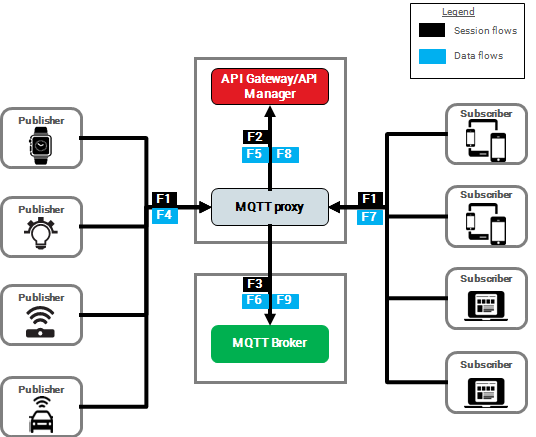
\includegraphics[width=14cm]{tex/bilder/2_grundlagen/axway-mqtt-proxy02_short.png}
        \captionof{figure}{Datenflow des Axway MQTT Proxies \cite{axway_2018}}
        \label{fig:axway-proxy}
    \end{figure}
    \begin{itemize}
        \item F1: Das \ac{IoT}-Gerät (Client) sendet eine Connect-Nachricht mit Benutzerdaten zum Proxy um sich damit zu verbinden
        \item F2: Die Benutzerdaten werden zum verifizieren dem API Gateway gesendet
        \item F3: Mit der Bestätigung vom Gateway wird die Session zum Proxy hergestellt.
        \item F4: Das Gerät sendet eine Nachricht an den Proxy.
        \item F5: Der Proxy verifiziert/ändert die Nachricht auf Basis der Gateway Regeln.
        \item F6: Die Nachricht wird an den externen Broker weitergeleitet.
        \item F7: Um nun eine Antwort zu erhalten sendet der Client eine Subscribe Nachricht an den Proxy
        \item F8: Der Proxy verifiziert/ändert die Nachricht auf Basis der Gateway Regeln.
        \item F9: Der Proxy leitet die Nachricht an den externen Broker weiter.
    \end{itemize}
    %Analyse der Lösung
    %Dieses Implementierung besitzt bereits die Möglichkeit, Daten abzufangen und den Inhalt auswerten zu können, so wie es ebenfalls in dieser Arbeit vorgesehen ist. Die gleichen Einschränkungen, welche die Lösung von Axway hat, wird auch in dieser Arbeit als Voraussetzung definiert: Es ist nicht ohne weiteres möglich ist, die Zertifikate, welche für eine TLS geschützte Verbindung mit dem Broker benötigt werden, zu erhalten. Da bei \ac{IoT} Geräten der Hersteller die Kontrolle über den Server und somit über die Zertifikate hat.
    %Was darüber hinaus jedoch nicht von API Management Plus angeboten wird, sind die folgenden Funktionen, welche im Rahmen eines Security Audits benötigt werden: 
    %\begin{itemize}
        %\item HTTP Schnittstelle zum senden selbst erzeugter Nachrichten an das gewählte Ziel.
        %\item Erneute versenden von bereits gesendeten Nachrichten um Nebeneffekte oder zustandsabhängige Funktionen zu erkennen.
        %\item Manuelle Manipulation der ausgehenden und ankommende Pakete.
    %\end{itemize}